%Mathematik 2
%Übungseinheit 3
%Hausübungen
%Aufgabe T1

\setcounter{T-section}{3}
\renewcommand*\thesection{T\Nummerierung{\arabic{T-section}}}
\section{Parallelprojektionen in die Aufrissebene}

\begin{center}
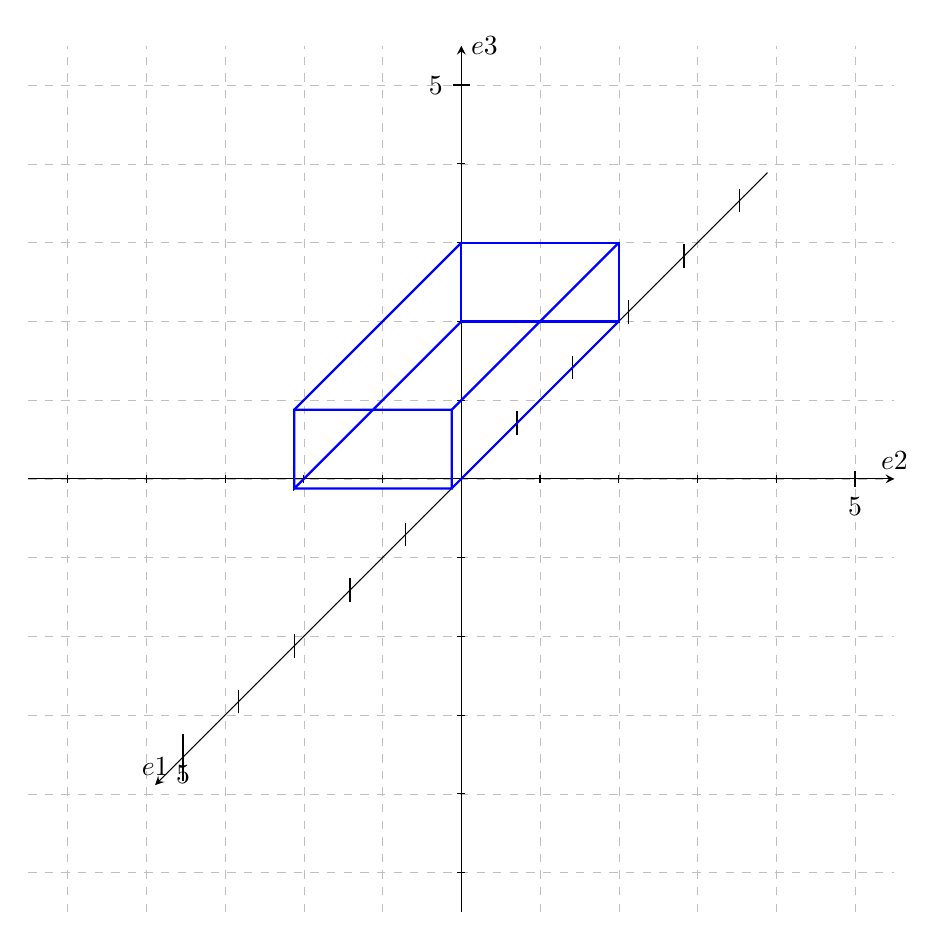
\begin{tikzpicture}[x=1cm,y=1cm,z=0.707cm,>=stealth]

\draw[step=1cm,lightgray,very thin,dashed] (-5.5,5.5) grid (5.5,-5.5);

% The axes
\draw[->] (xyz cs:x=-5.5) -- (xyz cs:x=5.5) node[above] {$e2$};
\draw[->] (xyz cs:y=-5.5) -- (xyz cs:y=5.5) node[right] {$e3$};
\draw[->] (xyz cs:z=5.5) -- (xyz cs:z=-5.5) node[above] {$e1$};
% The thin ticks

\foreach \coo in {-5,...,5}
{
	\draw (\coo,-1.5pt) -- (\coo,1.5pt);
	\draw (-1.5pt,\coo) -- (1.5pt,\coo);
	\draw (xyz cs:y=-0.15pt,z=\coo) -- (xyz cs:y=0.15pt,z=\coo);
}

% The thick ticks
\foreach \coo in {5}
{
	\draw[thick] (\coo,-3pt) -- (\coo,3pt) node[below=6pt] {\coo};
	\draw[thick] (-3pt,\coo) -- (3pt,\coo) node[left=6pt] {\coo};
	\draw[thick] (xyz cs:y=-0.3pt,z=-\coo) -- (xyz cs:y=0.3pt,z=-\coo) node[below=8pt] {\coo};
}

\draw[blue,thick] (xyz cs:x=0,y=2,z=0)--+(2,0,0)--+(2,1,0)--+(0,1,0)--cycle;
\draw[blue,thick] (xyz cs:x=0,y=2,z=0)--+(0,0,-3)--+(0,1,-3)--+(2,1,-3)--+(2,0,-3)--+(0,0,-3);
\draw[blue,thick] (xyz cs:x=2,y=2,z=0)--+(0,0,-3);
\draw[blue,thick] (xyz cs:x=0,y=3,z=0)--+(0,0,-3);
\draw[blue,thick] (xyz cs:x=2,y=3,z=0)--+(0,0,-3);

\end{tikzpicture}
\end{center}

\begin{center}
\begin{tikzpicture}[domain=0:2]
\draw[step=2cm,lightgray,very thin,dashed] (-7.5,7.5) grid (7.5,0);

\draw[->] (0,0) -- (7.5,0)
node[below right] {$x$};
\draw[->] (0,0) -- (0,7.5)
node[left] {$y$}; 
\draw[->] (0,0)--(-7.5,0)
node[left] {$z$};

\draw[blue,thick](0,4)--(4,4)--+(0,-2)--+(-4,-2)--cycle;
\draw[blue,thick](0,4)--(-6,4)--(-6,2)--(0,2);
\draw[blue,thick](-6,4)--(-6,2)--(-2,2)--(-2,4);


\end{tikzpicture}
\end{center}
